% Options for packages loaded elsewhere
\PassOptionsToPackage{unicode}{hyperref}
\PassOptionsToPackage{hyphens}{url}
%
\documentclass[
]{book}
\usepackage{lmodern}
\usepackage{amssymb,amsmath}
\usepackage{ifxetex,ifluatex}
\ifnum 0\ifxetex 1\fi\ifluatex 1\fi=0 % if pdftex
  \usepackage[T1]{fontenc}
  \usepackage[utf8]{inputenc}
  \usepackage{textcomp} % provide euro and other symbols
\else % if luatex or xetex
  \usepackage{unicode-math}
  \defaultfontfeatures{Scale=MatchLowercase}
  \defaultfontfeatures[\rmfamily]{Ligatures=TeX,Scale=1}
\fi
% Use upquote if available, for straight quotes in verbatim environments
\IfFileExists{upquote.sty}{\usepackage{upquote}}{}
\IfFileExists{microtype.sty}{% use microtype if available
  \usepackage[]{microtype}
  \UseMicrotypeSet[protrusion]{basicmath} % disable protrusion for tt fonts
}{}
\makeatletter
\@ifundefined{KOMAClassName}{% if non-KOMA class
  \IfFileExists{parskip.sty}{%
    \usepackage{parskip}
  }{% else
    \setlength{\parindent}{0pt}
    \setlength{\parskip}{6pt plus 2pt minus 1pt}}
}{% if KOMA class
  \KOMAoptions{parskip=half}}
\makeatother
\usepackage{xcolor}
\IfFileExists{xurl.sty}{\usepackage{xurl}}{} % add URL line breaks if available
\IfFileExists{bookmark.sty}{\usepackage{bookmark}}{\usepackage{hyperref}}
\hypersetup{
  pdftitle={Accounting for commercial data without reallocationg the catches.},
  pdfauthor={MP Etienne},
  hidelinks,
  pdfcreator={LaTeX via pandoc}}
\urlstyle{same} % disable monospaced font for URLs
\usepackage{color}
\usepackage{fancyvrb}
\newcommand{\VerbBar}{|}
\newcommand{\VERB}{\Verb[commandchars=\\\{\}]}
\DefineVerbatimEnvironment{Highlighting}{Verbatim}{commandchars=\\\{\}}
% Add ',fontsize=\small' for more characters per line
\usepackage{framed}
\definecolor{shadecolor}{RGB}{248,248,248}
\newenvironment{Shaded}{\begin{snugshade}}{\end{snugshade}}
\newcommand{\AlertTok}[1]{\textcolor[rgb]{0.94,0.16,0.16}{#1}}
\newcommand{\AnnotationTok}[1]{\textcolor[rgb]{0.56,0.35,0.01}{\textbf{\textit{#1}}}}
\newcommand{\AttributeTok}[1]{\textcolor[rgb]{0.77,0.63,0.00}{#1}}
\newcommand{\BaseNTok}[1]{\textcolor[rgb]{0.00,0.00,0.81}{#1}}
\newcommand{\BuiltInTok}[1]{#1}
\newcommand{\CharTok}[1]{\textcolor[rgb]{0.31,0.60,0.02}{#1}}
\newcommand{\CommentTok}[1]{\textcolor[rgb]{0.56,0.35,0.01}{\textit{#1}}}
\newcommand{\CommentVarTok}[1]{\textcolor[rgb]{0.56,0.35,0.01}{\textbf{\textit{#1}}}}
\newcommand{\ConstantTok}[1]{\textcolor[rgb]{0.00,0.00,0.00}{#1}}
\newcommand{\ControlFlowTok}[1]{\textcolor[rgb]{0.13,0.29,0.53}{\textbf{#1}}}
\newcommand{\DataTypeTok}[1]{\textcolor[rgb]{0.13,0.29,0.53}{#1}}
\newcommand{\DecValTok}[1]{\textcolor[rgb]{0.00,0.00,0.81}{#1}}
\newcommand{\DocumentationTok}[1]{\textcolor[rgb]{0.56,0.35,0.01}{\textbf{\textit{#1}}}}
\newcommand{\ErrorTok}[1]{\textcolor[rgb]{0.64,0.00,0.00}{\textbf{#1}}}
\newcommand{\ExtensionTok}[1]{#1}
\newcommand{\FloatTok}[1]{\textcolor[rgb]{0.00,0.00,0.81}{#1}}
\newcommand{\FunctionTok}[1]{\textcolor[rgb]{0.00,0.00,0.00}{#1}}
\newcommand{\ImportTok}[1]{#1}
\newcommand{\InformationTok}[1]{\textcolor[rgb]{0.56,0.35,0.01}{\textbf{\textit{#1}}}}
\newcommand{\KeywordTok}[1]{\textcolor[rgb]{0.13,0.29,0.53}{\textbf{#1}}}
\newcommand{\NormalTok}[1]{#1}
\newcommand{\OperatorTok}[1]{\textcolor[rgb]{0.81,0.36,0.00}{\textbf{#1}}}
\newcommand{\OtherTok}[1]{\textcolor[rgb]{0.56,0.35,0.01}{#1}}
\newcommand{\PreprocessorTok}[1]{\textcolor[rgb]{0.56,0.35,0.01}{\textit{#1}}}
\newcommand{\RegionMarkerTok}[1]{#1}
\newcommand{\SpecialCharTok}[1]{\textcolor[rgb]{0.00,0.00,0.00}{#1}}
\newcommand{\SpecialStringTok}[1]{\textcolor[rgb]{0.31,0.60,0.02}{#1}}
\newcommand{\StringTok}[1]{\textcolor[rgb]{0.31,0.60,0.02}{#1}}
\newcommand{\VariableTok}[1]{\textcolor[rgb]{0.00,0.00,0.00}{#1}}
\newcommand{\VerbatimStringTok}[1]{\textcolor[rgb]{0.31,0.60,0.02}{#1}}
\newcommand{\WarningTok}[1]{\textcolor[rgb]{0.56,0.35,0.01}{\textbf{\textit{#1}}}}
\usepackage{longtable,booktabs}
% Correct order of tables after \paragraph or \subparagraph
\usepackage{etoolbox}
\makeatletter
\patchcmd\longtable{\par}{\if@noskipsec\mbox{}\fi\par}{}{}
\makeatother
% Allow footnotes in longtable head/foot
\IfFileExists{footnotehyper.sty}{\usepackage{footnotehyper}}{\usepackage{footnote}}
\makesavenoteenv{longtable}
\usepackage{graphicx,grffile}
\makeatletter
\def\maxwidth{\ifdim\Gin@nat@width>\linewidth\linewidth\else\Gin@nat@width\fi}
\def\maxheight{\ifdim\Gin@nat@height>\textheight\textheight\else\Gin@nat@height\fi}
\makeatother
% Scale images if necessary, so that they will not overflow the page
% margins by default, and it is still possible to overwrite the defaults
% using explicit options in \includegraphics[width, height, ...]{}
\setkeys{Gin}{width=\maxwidth,height=\maxheight,keepaspectratio}
% Set default figure placement to htbp
\makeatletter
\def\fps@figure{htbp}
\makeatother
\setlength{\emergencystretch}{3em} % prevent overfull lines
\providecommand{\tightlist}{%
  \setlength{\itemsep}{0pt}\setlength{\parskip}{0pt}}
\setcounter{secnumdepth}{5}
\usepackage{booktabs}

\newcommand{\point}{\mathcal{P}}
\usepackage[]{natbib}
\bibliographystyle{apalike}

\title{Accounting for commercial data without reallocationg the catches.}
\author{MP Etienne}
\date{2021-02-19}

\begin{document}
\maketitle

{
\setcounter{tocdepth}{1}
\tableofcontents
}
\hypertarget{model-presentation}{%
\chapter{Model presentation}\label{model-presentation}}

\hypertarget{log-normal-parametrization}{%
\section{Log Normal parametrization}\label{log-normal-parametrization}}

Many different parametrizations of the log normal exist, We have to choose the most convenient for our purpose

\hypertarget{version-1}{%
\subsection{Version 1}\label{version-1}}

\begin{equation} 
  D \sim \mathcal{LN} (\rho, \sigma^2) \Longleftrightarrow D =e^{\rho + \sigma N}, \ N\sim \mathcal{N}(0,1) .
  \label{eq:LNv1}
\end{equation}

In this parametrization
\[E(D) = e^{\rho +\frac{\sigma^2}{2}},\quad Var(D) = \left(e^{\sigma^2}-1\right) e^{2\rho + \sigma^2}\]

\hypertarget{version-2}{%
\subsection{Version 2}\label{version-2}}

\begin{equation} 
  D \sim \mathcal{LN} (\nu, \sigma^2) \Longleftrightarrow D =\mu e^{\sigma N}, \ N\sim \mathcal{N}(0,1) .
  \label{eq:LNv2}
\end{equation}

In this parametrization
\[E(D) = \nu e^{\frac{\sigma^2}{2}},\quad Var(D) = \nu^2 \left(e^{\sigma^2}-1\right) e^{ \sigma^2}\]

\hypertarget{version-3-the-mean-of-the-log-normal-is-the-actual-parameter}{%
\subsection{Version 3, the mean of the log normal is the actual parameter}\label{version-3-the-mean-of-the-log-normal-is-the-actual-parameter}}

\begin{equation} 
  D \sim \mathcal{LN} (\mu, \sigma^2) \Longleftrightarrow D =\mu e^{\sigma N- \frac{\sigma^2}{2}}, \ N\sim \mathcal{N}(0,1) .
  \label{eq:LNv3}
\end{equation}

In this parametrization
\[E(D) = \mu ,\quad Var(D) = \mu^2 \left(e^{\sigma^2}-1\right). \]
With this parametrization,

\[D \sim\mathcal{LN}\left ( E(D), \ln\left\lbrace Var(D)/E(D)^2 +1\right\rbrace\right ).\]
We will use this last parametrization throughout the paper.

\hypertarget{model}{%
\section{Model}\label{model}}

The model proposed by Baptiste has a hierarchical structure with three main components

\begin{itemize}
\tightlist
\item
  the biomass latent field \(S\), representing the spatial repartition of biomass:
\end{itemize}

\begin{equation} 
  S(x)  = \exp{ \left \lbrace \alpha_S + \Gamma_S(x)^\intercal \beta_S +\delta(x)\right \rbrace}
  \label{eq:latent}
\end{equation}

\begin{itemize}
\tightlist
\item
  the preferential sampling density, defined conditionnally to \(S\):
\end{itemize}

\begin{equation} 
  \lambda(x)  = \exp{ \left \lbrace \alpha_X + b \log{\left \lbrace S(x)\right\rbrace} + \Gamma_X(x)^\intercal \beta_X +\eta(x)\right \rbrace}
  \label{eq:pref}
\end{equation}

\begin{itemize}
\tightlist
\item
  and finally, the observations are defined at the VMS ping scale. \(Y_i\) stands for the CPUE at location \(x_i\) and is defined conditionnaly on the Poisson process and the biomass latent field \(S\):
\end{itemize}

\begin{align*} 
  Y_i  &= C_i Z_i,    \label{eq:obs}\\ 
  C_i &\sim \mathcal{B}(1-p_i), \mbox{ with } p_i = \exp{ \left \lbrace  - e^{\xi \mu(x_i) }\right \rbrace}, \nonumber  \\
  Z_i &\sim \mathcal{LN}( \frac{\mu(x_i)}{1-p_i}, \sigma^2),\nonumber \\
  \mu(x_i) &= q S(x_i).\nonumber \\
\end{align*}

\hypertarget{potential-limitation}{%
\section{Potential limitation}\label{potential-limitation}}

The information regarding the catch is not known at the fishing point level (VMS ping) but at the statistical unit, as recorded in the logbook.
The available information on the commercial catch is the declaration \(D_j\) at the statistical unit level and the VMS ping location \((x_{j1}, \ldots x_{jn_j})\). \(D_j\) is the sum of all individuals catch at the \(n_j\) visited fishing points:

\begin{equation*}
  D_{j} = \sum_{i \in  \mathcal{P}_j} Y_i,
\end{equation*}

\(\mathcal{P}_j\) being the vector of all fishing events associated with the logbook entry \(j\).

This diffculty is currently addressed by reallocating the total catch to individual fishing events with a simple proportionality rule:
\[\tilde{Y_i} = \frac{1}{|\mathcal{P}_j|} D_j.\]

This is not completely satisfactory as it might introduce some bias is the total biomass estimation as well as its spatial repetition.

\hypertarget{is-is-a-real-limitation}{%
\section{Is is a real limitation ?}\label{is-is-a-real-limitation}}

A strategy to answer this question would be

\begin{enumerate}
\def\labelenumi{\arabic{enumi}.}
\tightlist
\item
  Simulation study to understand when this reallocation is problematic
\item
  A new observation model at the statitical unit level
\item
  Does this new model improves the estimation ?
\end{enumerate}

\hypertarget{effects}{%
\chapter{A simulation study to explore the effects of the reallocation}\label{effects}}

Put the stats project here

\hypertarget{a-new-model-for-commrecial-data}{%
\chapter{A new model for commrecial data}\label{a-new-model-for-commrecial-data}}

As mentionned in the introduction, every commercial catch is reported by statistical area/vessel/gear and correspond potentially to several VMS ping.
Let's denote \(D_j\) a reported catch associated to \(|\mathcal{P}_j|\) VMS ping at positions \(\left\lbrace x_i, i\in \mathcal{P}_j \right\rbrace\). \(D_j\) is the sum of all individuals catch at the \(n_j\) visited fishing points:

\begin{equation}
  D_{j} = \sum_{i \in  C_j} Y_i,
  \label{eq:logbook}
\end{equation}

\(C_j\) begin the vector of all fishing events associated with the logbook entry \(j\).

This diffculty is currently addressed by reallocating the total catch to individual fishing events with a simple proportionality rule:
\[\tilde{Y_i} = \frac{1}{|C_j|} D_j.\]

\(\tilde{Y}_i\) is the assumed to follow the observation model defined \eqref{eq:logbook}.

A more satisfying solution would consist in deriving the distribution of \(D_j\) from the distribution of \(Y_i\). However the sum of a mixture of delta lognormal random variables do not resume in a nice known distribution.

An alternative would be to fit a delta lognormal model whose proportion of zero and the two first moments coincide i.e

\begin{align}
P(D_j = 0 \vert S, X) & = \prod_{i\in \mathcal{P}_j} P(Y_i = 0 \vert S, X),\nonumber \\
                      & = \exp{ \left \lbrace- \sum_{i\in \mathcal{P}_j} e^{\xi S(x_i)}\right \rbrace}.
\end{align}

The expected catch biomass is defined by \(E(D_j) = \sum_{i\in \mathcal{P}_j} E(C_i Z_i).\)

As \(C_i\) and \(Z_i\) are assumed to be independant

\begin{align}
E(D_j) & = \sum_{i\in \mathcal{P}_j} E(C_i Z_i),\nonumber \\
& = \sum_{i\in \mathcal{P}_j} (1-p_i) \frac{\mu(x_i)}{1-p_i}, \nonumber \\
& = \sum_{i\in \mathcal{P}_j} \mu(x_i). \label{eq:newobs}
\end{align}

Regarding the variance

\[Var(D_j)  = \sum_{i\in \mathcal{P}_j} Var(C_i Z_i).\]

We are the lead to compute the Variance of \(C_i Z_i\).

\begin{align*}
Var(C_i Z_i) & = E( var(C_i Z_i \vert C_i) )  + Var( E(C_i Z_i \vert C_i) ),\\
& = Var(Z_i) E(C_i^2) + Var ( E(Z_i) C_i),\\
& = Var(Z_i) (1-p_i) + E(Z_i)^2 p_i (1-p_i)
\end{align*}

\hypertarget{numerical-illustration}{%
\section{Numerical illustration}\label{numerical-illustration}}

\hypertarget{precising-the-notation}{%
\subsection{Precising the notation}\label{precising-the-notation}}

As mentioned in Equation \eqref{eq:LNv3}, \(Y\sim \mathcal{LN}(\mu, \sigma^2)\) stands a lognormal distribution such that \(E(Y) = \mu\) and \(Var(log(Y)) = \sigma^2\).

An alterntive commun specificication denotes \(Y \sim LN(\rho, \sigma)\) if \(E(log(Y))=\rho\) and \(Var(log(Y)) = \sigma^2\)

Look at the the sum of n lognormal distribution

The code below is an helper to go back and forth between the different parametrizations.

\begin{Shaded}
\begin{Highlighting}[]
\NormalTok{log_normal_variance2 <-}\StringTok{ }\ControlFlowTok{function}\NormalTok{(rho, sigma)\{}
\NormalTok{  ( }\KeywordTok{exp}\NormalTok{(sigma}\OperatorTok{^}\DecValTok{2}\NormalTok{) }\OperatorTok{-}\StringTok{ }\DecValTok{1}\NormalTok{ ) }\OperatorTok{*}\StringTok{ }\KeywordTok{exp}\NormalTok{(}\DecValTok{2}\OperatorTok{*}\StringTok{ }\NormalTok{rho  }\OperatorTok{+}\StringTok{ }\NormalTok{sigma}\OperatorTok{^}\DecValTok{2}\NormalTok{)}
\NormalTok{\}}

\NormalTok{LN_rho2mu <-}\StringTok{ }\ControlFlowTok{function}\NormalTok{(rho, sigma)\{}
   \KeywordTok{exp}\NormalTok{(rho}\OperatorTok{+}\StringTok{ }\NormalTok{sigma}\OperatorTok{^}\DecValTok{2} \OperatorTok{/}\DecValTok{2}\NormalTok{ )}
\NormalTok{\}}

\NormalTok{LN_mu2rho <-}\StringTok{ }\ControlFlowTok{function}\NormalTok{(mu, sigma)\{}
   \KeywordTok{log}\NormalTok{(mu) }\OperatorTok{-}\StringTok{ }\NormalTok{sigma}\OperatorTok{^}\DecValTok{2} \OperatorTok{/}\DecValTok{2}
\NormalTok{\}}

\NormalTok{log_normal_variance1 <-}\StringTok{ }\ControlFlowTok{function}\NormalTok{(mu, sigma)\{}
  \KeywordTok{log_normal_variance2}\NormalTok{(}\KeywordTok{LN_mu2rho}\NormalTok{(mu, sigma), sigma)}
\NormalTok{\}}

\NormalTok{log_normal_mean2 <-}\StringTok{ }\ControlFlowTok{function}\NormalTok{(rho, sigma)\{}
   \KeywordTok{exp}\NormalTok{( rho }\OperatorTok{+}\StringTok{ }\NormalTok{sigma}\OperatorTok{^}\DecValTok{2}\OperatorTok{/}\DecValTok{2}\NormalTok{ )}
\NormalTok{\}}
\end{Highlighting}
\end{Shaded}

\hypertarget{n-2}{%
\subsection{n = 2}\label{n-2}}

\begin{Shaded}
\begin{Highlighting}[]
\KeywordTok{set.seed}\NormalTok{(}\DecValTok{1234}\NormalTok{)}
\NormalTok{n <-}\StringTok{ }\DecValTok{2}
\NormalTok{rho <-}\StringTok{ }\KeywordTok{rnorm}\NormalTok{(n, }\DataTypeTok{mean =} \DecValTok{0}\NormalTok{, }\DataTypeTok{sd =} \DecValTok{1}\NormalTok{ )}
\NormalTok{sigma <-}\StringTok{ }\DecValTok{01}
\end{Highlighting}
\end{Shaded}

We are ready to look at the sum of 2 lognormal random variables with mean 0.493, 2.176 and variance 0.418, 8.135 .

\begin{Shaded}
\begin{Highlighting}[]
\NormalTok{n_sim <-}\StringTok{ }\DecValTok{1000}
\NormalTok{dta <-}\StringTok{ }\NormalTok{rho }\OperatorTok\StringTok{ }\KeywordTok{map}\NormalTok{(}\ControlFlowTok{function}\NormalTok{(x)\{ }\KeywordTok{exp}\NormalTok{(}\KeywordTok{rnorm}\NormalTok{(}\DataTypeTok{n =}\NormalTok{ n_sim, }\DataTypeTok{mean =}\NormalTok{ x, }\DataTypeTok{sd =}\NormalTok{ sigma))\}) }\OperatorTok\StringTok{ }
\StringTok{   }\KeywordTok{map_df}\NormalTok{(}
         \OperatorTok{~}\StringTok{ }\KeywordTok{data_frame}\NormalTok{(}\DataTypeTok{x =}\NormalTok{ .x), }
         \DataTypeTok{.id =} \StringTok{"dist"}
\NormalTok{     ) }
\end{Highlighting}
\end{Shaded}

\begin{verbatim}
## Warning: `data_frame()` is deprecated as of tibble 1.1.0.
## Please use `tibble()` instead.
## This warning is displayed once every 8 hours.
## Call `lifecycle::last_warnings()` to see where this warning was generated.
\end{verbatim}

\begin{Shaded}
\begin{Highlighting}[]
\NormalTok{p <-}\StringTok{ }\NormalTok{dta }\OperatorTok\StringTok{ }\KeywordTok{ggplot}\NormalTok{() }\OperatorTok{+}\StringTok{ }\KeywordTok{geom_histogram}\NormalTok{(}\KeywordTok{aes}\NormalTok{(}\DataTypeTok{x=}\NormalTok{x, }\DataTypeTok{y=}\NormalTok{..density.., }\DataTypeTok{fill =}\NormalTok{ dist), }\DataTypeTok{position=}\StringTok{"identity"}\NormalTok{, )}

\NormalTok{p}
\end{Highlighting}
\end{Shaded}

\begin{verbatim}
## `stat_bin()` using `bins = 30`. Pick better value with `binwidth`.
\end{verbatim}

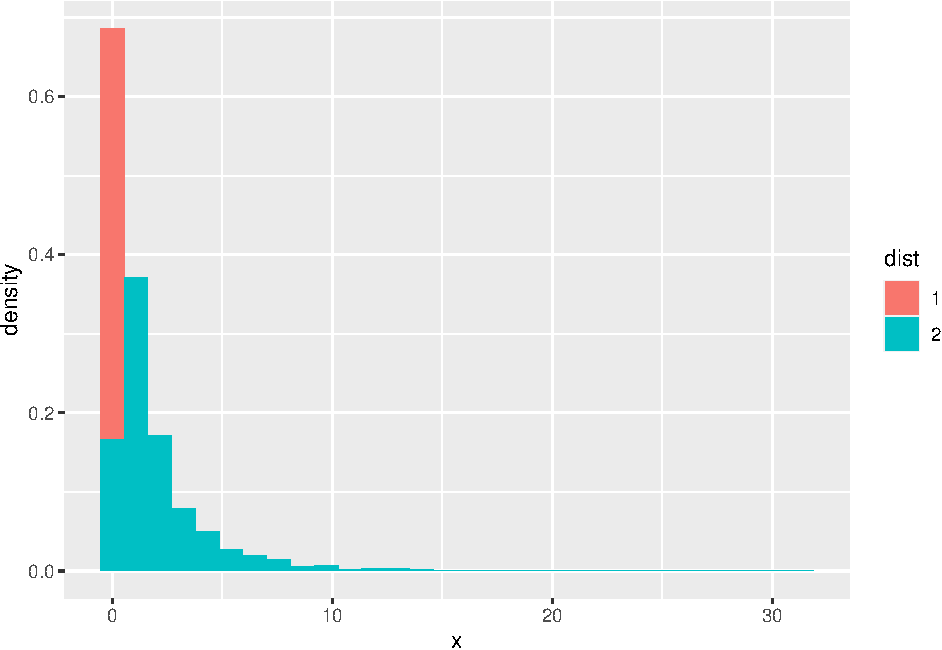
\includegraphics{2021_realloc_files/figure-latex/sample_2_lognorm-1.pdf}

\begin{Shaded}
\begin{Highlighting}[]
\NormalTok{sum_dta <-}\StringTok{ }\NormalTok{dta }\OperatorTok\StringTok{ }\KeywordTok{group_by}\NormalTok{(dist) }\OperatorTok\StringTok{ }
\StringTok{  }\KeywordTok{mutate}\NormalTok{(}\DataTypeTok{id =} \KeywordTok{row_number}\NormalTok{()) }\OperatorTok\StringTok{ }
\StringTok{  }\KeywordTok{pivot_wider}\NormalTok{(}\DataTypeTok{names_from =}\NormalTok{ dist,    }\DataTypeTok{names_glue =} \StringTok{"dist_\{dist\}"}\NormalTok{,}
 \DataTypeTok{values_from =}\NormalTok{x) }\OperatorTok\StringTok{ }
\StringTok{  }\KeywordTok{mutate}\NormalTok{( }\DataTypeTok{D =} \KeywordTok{rowSums}\NormalTok{(.[}\KeywordTok{grep}\NormalTok{(}\StringTok{"dist_"}\NormalTok{, }\KeywordTok{names}\NormalTok{(.))]))}

\NormalTok{sum_dta }\OperatorTok\StringTok{ }\KeywordTok{ggplot}\NormalTok{() }\OperatorTok{+}\StringTok{ }\KeywordTok{geom_histogram}\NormalTok{(}\KeywordTok{aes}\NormalTok{(}\DataTypeTok{x=}\NormalTok{D), }\DataTypeTok{position=}\StringTok{"identity"}\NormalTok{)}
\end{Highlighting}
\end{Shaded}

\begin{verbatim}
## `stat_bin()` using `bins = 30`. Pick better value with `binwidth`.
\end{verbatim}

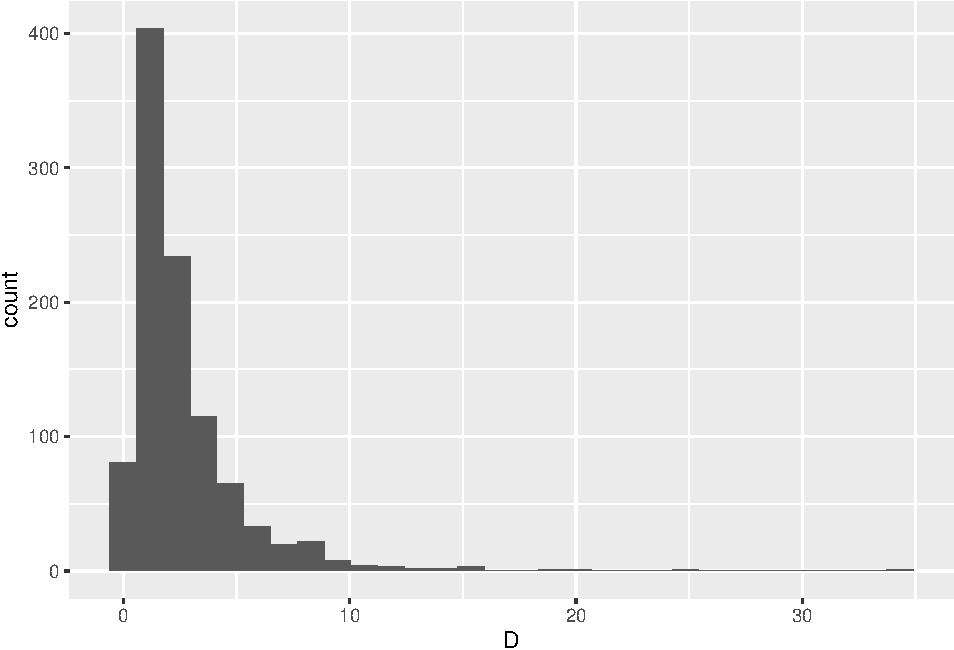
\includegraphics{2021_realloc_files/figure-latex/sample_2_lognorm-2.pdf}

\begin{Shaded}
\begin{Highlighting}[]
\NormalTok{mu_sum <-}\StringTok{ }\KeywordTok{sum}\NormalTok{(}\KeywordTok{LN_rho2mu}\NormalTok{(rho, sigma))}
\NormalTok{S2_sum <-}\StringTok{ }\KeywordTok{sum}\NormalTok{(}\KeywordTok{log_normal_variance2}\NormalTok{(rho, sigma))}
\NormalTok{sigma_sum =}\StringTok{ }\KeywordTok{sqrt}\NormalTok{( S2_sum}\OperatorTok{/}\NormalTok{mu_sum}\OperatorTok{^}\DecValTok{2} \OperatorTok{+}\DecValTok{1}\NormalTok{)}

\NormalTok{sum_density <-}\StringTok{ }\KeywordTok{tibble}\NormalTok{(}\DataTypeTok{x  =} \KeywordTok{seq}\NormalTok{(}\FloatTok{0.001}\NormalTok{, }\KeywordTok{max}\NormalTok{(sum_dta}\OperatorTok{$}\NormalTok{D), }\FloatTok{0.1}\NormalTok{)) }\OperatorTok\StringTok{ }
\StringTok{  }\KeywordTok{mutate}\NormalTok{(}\DataTypeTok{log_x =} \KeywordTok{log}\NormalTok{(x), }
         \DataTypeTok{dens =} \KeywordTok{dnorm}\NormalTok{(log_x, }
                         \DataTypeTok{mean=}\KeywordTok{LN_mu2rho}\NormalTok{(mu_sum, sigma_sum), }
                         \DataTypeTok{sd =}\NormalTok{ sigma_sum))}

\NormalTok{p }\OperatorTok{+}\StringTok{ }\KeywordTok{geom_line}\NormalTok{(}\DataTypeTok{data=}\NormalTok{ sum_density, }\KeywordTok{aes}\NormalTok{(}\DataTypeTok{x=}\NormalTok{x, }\DataTypeTok{y =}\NormalTok{dens))}
\end{Highlighting}
\end{Shaded}

\begin{verbatim}
## `stat_bin()` using `bins = 30`. Pick better value with `binwidth`.
\end{verbatim}

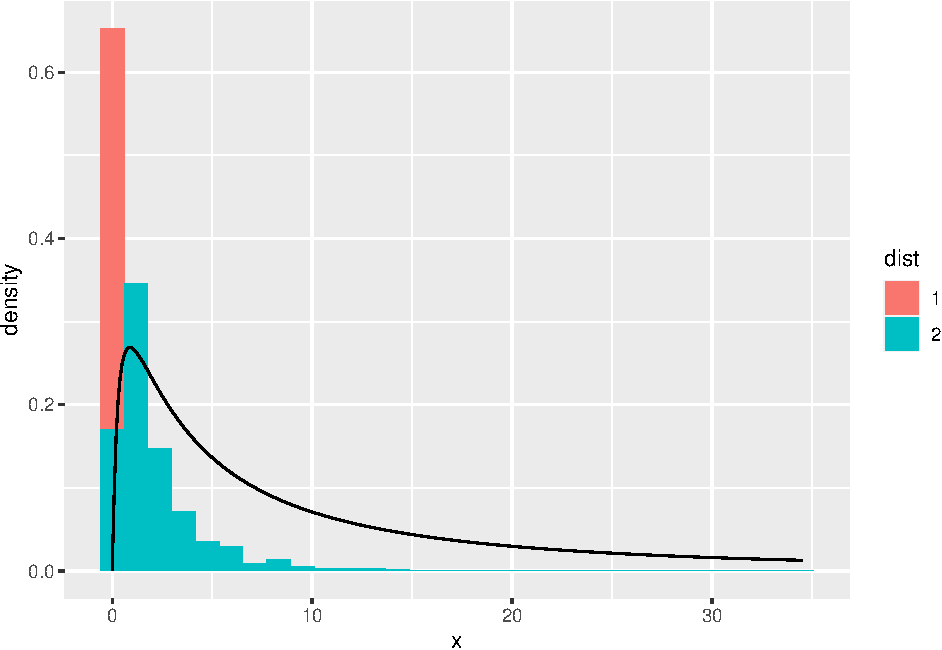
\includegraphics{2021_realloc_files/figure-latex/sample_2_lognorm-3.pdf}

La moyenne théorique attendue est 2.6689604 et la moyenne empirique vaut 2.6173234, la variance théorique vaut 57.2084894 et la variance empirique vaut 7.0105572.

  \bibliography{book.bib,packages.bib}

\end{document}
